\documentclass[11pt]{article}

\usepackage[utf8]{inputenc}
\usepackage[english]{babel}
\usepackage{natbib}
\usepackage[T1]{fontenc}
\usepackage{setspace}
\usepackage{graphicx}
\usepackage{hyperref}
\usepackage[top=3.5cm,left=3.5cm,right=3.5cm,bottom=3.5cm]{geometry} % 'showframe' to see borders

\providecommand{\keywords}[1] {
  \small
  \textbf{\textit{Keywords---}} #1
}

\graphicspath{ {diagram/} }

\title{\vspace{2cm}\textbf{Information and Network Security}\\6G6Z1012}
\author{Joshua Michael Ephraim Bridge\\14032908\\Software Engineering}

\pagestyle{headings}

\begin{document}

  \maketitle

  \vspace{1cm}

  \begin{abstract}
    In this report a solution is proposed for creating a secure network within a financial company which is much more defended from both internal and external attacks. Some of the technologies proposed are re-used for greater cost-effectiveness (such as IPSec tunnel) without compromising on security. Multiple vulnerabilities \& attacks with the current network layout are highlighted and solutions for each are clearly defined. Finally, every additional requirement from the company is met with a cost-effective solution, again through re-use of technologies.
  \end{abstract}

  \vspace{0.5cm}

  \keywords{IPSec tunnel (VPN), Application-level Gateway, IDS (Network), SFTP}

  \newpage

  % \tableofcontents

  \section{System Analysis (Vulnerabilities \& Attacks)}
    \subsection{Insecure IP packets}
      At the moment, the branches communicate to the headquarters over the internet in an insecure way. As the packets being sent over the internet are not protected, anyone could read the contents of these messages and potentially use them to attack the system. Any router or system that lies in the network path between each branch and the headquarters could intercept any message sent between them and possibly modify, remove or replay that message.

      \paragraph{Replay Attack}
        The current network is very susceptible to a replay attack with its user/password system. As there is no underlying security protocol to protect messages over the internet, a packet sniffer could be used to listen for a valid sign-in message and then that message could be re-sent by an attacker to gain access to the system \citep{owaspReplayAttack}.

    \subsection{Internal Access Control}
      A major issue with the current network layout is that all devices in each location are grouped together within the same LAN, so any computer/server can access every other computer/server. There is no access control which could prevent resources being accessed by users who should not be able to.

      \paragraph{Internal Malicious Access}
        Either an employee with internal network access or an outside attacker who has gained access to the network is able to access all of the resources within any location. This allows the possibility of a whole host of attacks such as offline dictionary attacks \& DNS cache poisoning.

    \subsection{User/Password Authentication}
      A user/password system is unsuitable for secure authentication when connecting over the internet. Usernames and passwords for users are often very simple for the sake of being able to remember them, therefore this makes them much more susceptible to being guessed by an attacker.

      \paragraph{Offline Dictionary Attack}
        If an attacker manages to get into the database containing all company usernames and passwords and there is no encryption on the passwords, then they can easily make a copy of all of these records and then could use them to hijack any system on the network without effort \citep{capecDictionary}.

    \subsection{Insecure FTP Server}
      The current FTP server is serving with unprotected traffic, which is easily exploitable and a very critical vulnerability when the company is dealing with financial information.

      \paragraph{Packet sniffing}
        Attackers can scan network traffic to easily pick up FTP login passwords sent in plain text, furthermore they can see the files being transferred and make a copy of any file. This can be done with free software such as Wireshark (\url{https://www.wireshark.org}).

    \subsection{Unprotected DNS}
      The DNS server at the headquarters is currently located within the same LAN as the public facing servers and the office workstations. Therefore if any of these devices were to be compromised then the DNS server is very susceptible to being attacked.

      \paragraph{DNS cache poisoning}
        Due to the current network design, once an attacker has gained entry to an employee computer via either a Replay or Dictionary attack it is possible to then reach the DNS server via the LAN and poison its cache \citep{son2010hitchhiker}. It would therefore be possible to redirect any authentication traffic to an attacker-controlled server and collect the passwords of every user that tried to log in while the cache is poisoned.

    \section{Secure Network Design Proposal}
      \subsection{Attack Prevention}
        In order to protect against the attacks I have identified, I suggest that the following technologies be implemented. In \textbf{bold} are the vulnerabilities/attacks which are being prevented.

        \subsubsection{IPsec-ESP (VPN)} \label{ipsec}
          In order to protect against \textbf{Replay attacks}, an IPsec tunnel is an ideal solution for maintaining message authenticity \citep{ncsc2016IPSec}. When deployed in ESP mode, all devices connecting remotely to the main network have a secure connection which can not be interfered with by attackers. Using network sniffing tools on this connection would only show encrypted packets with an IP destination and re-sending the same packet would not work due to the TTL (Time to live) header which specifically protects against replay attacks. This method is suitable as the organisation already has the DNS infrastructure required for setting up a VPN, it would only require replacement of the office boundary routers from the ones supplied by the ISP in order to handle the VPN traffic.

        \subsubsection{Application-level Gateway} \label{app-gateway}
          An application-level Gateway would be an ideal solution for protecting against \textbf{Internal Malicious Access} and therefore also protecting against \textbf{DNS Cache Poisoning} \& \textbf{Offline Dictionary Attacks}. This is due to the fact that if an attacker can not gain access the internal network then it is not possible for them to even begin more specific attacks such as the two mentioned previously. The networks within the headquarters should be split up into DMZs separated by firewalls, where only certain users are permitted to cross these zones for certain application uses (This can be seen in fig. \ref{fig:network-diagram}). For example if an outside attacker has managed to gain access to an account within the network, they still will not be able to access the DNS server due to not having the correct authentication to access the server.

        \subsubsection{SFTP (Secure File Transfer Protocol)}
          To protect against \textbf{Insecure FTP}, a more secure file transfer protocol implementation is ideal. While internet traffic would be protected from IPSec VPN, within the network file transfers would still be insecure. SFTP is an extension of SSH (Secure Shell) which allows for secure transfer of files over any network \citep{sshSFTP}. This is relatively simple to set up and does not interfere with any firewall, as it only requires a single port (22) to work. This makes it a much easier solution than FTPS (FTP Secure) which requires many ports which are difficult to manage \citep{ga2011sftp}. Many FTP clients support SFTP such as Filezilla (\url{https://filezilla-project.org}) and WinSCP (\url{https://winscp.net/}) so updating to this new protocol should not require much effort.

          \begin{figure}[h]
            \centering
            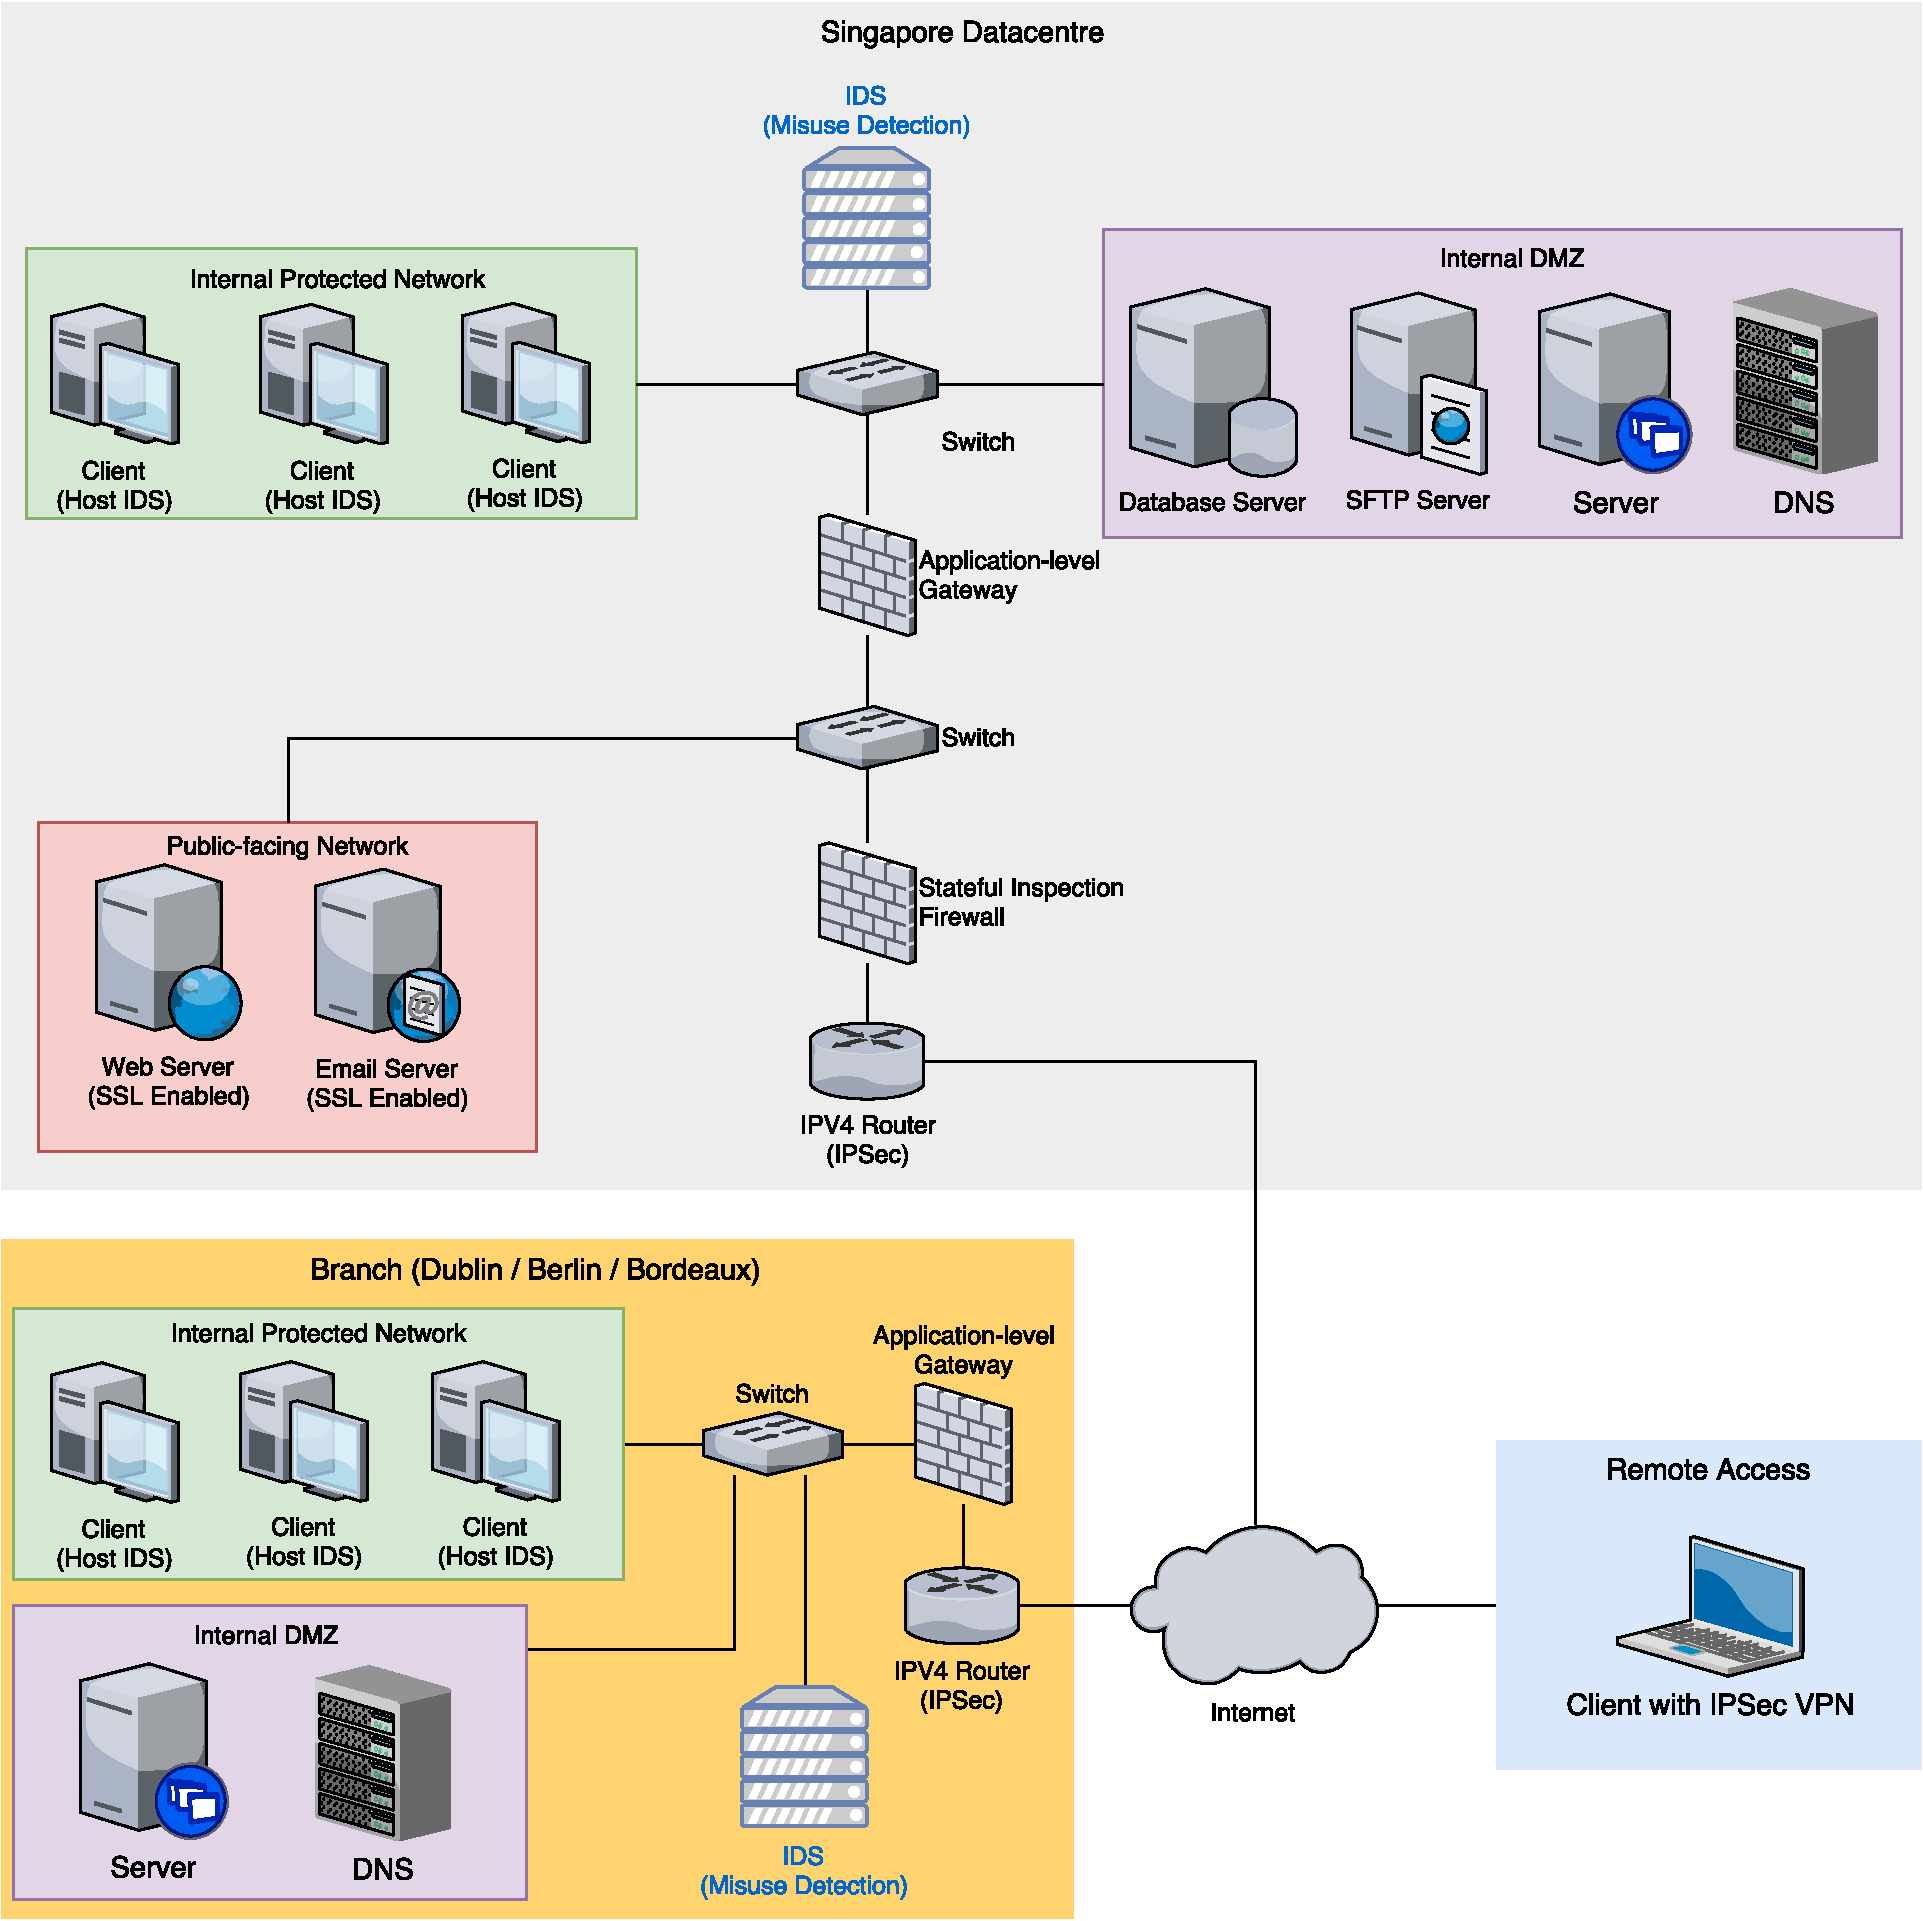
\includegraphics[width=13cm]{network-diagram.pdf}
            \caption{Network diagram}
            \label{fig:network-diagram}
          \end{figure}

      \subsection{Additional Requirements}
        Below are the solutions I propose for each of the additional requirements of the company.

        \subsubsection{Authentication} \label{auth}
          For authenticating users, I would suggest that a more secure form of the user/password system be implemented such as password Hash \& Salt. A salt of 64 bytes is the standard recommended size if allowed by the storage mechanism \citep{owaspSalt}. A salt dramatically slows down \textbf{Offline Dictionary Attacks} as each attempted password crack must be re-computed for each different salt. Therefore it is suggested to use a unique salt for each password and not a single re-used salt. This would not require huge amounts of work as the user system is already in place. Additionally, this would make sure the passwords are not in plain-text when sent over the network, stopping them from being picked up by an attacker using a packet sniffer.

        \subsubsection{Access Control}
          Access control could easily be managed by the application-level gateway described in section \ref{app-gateway}. The gateway is capable of understanding which users have access to which resources and can stop the packets from reaching the intended destination if the user does not have the correct permissions as specified in its policy fields \citep{openAppGateway}.

        \subsubsection{Site-to-site Connection} \label{ipsec2}
          An IPsec VPN (as mentioned in section \ref{ipsec}) would provide a secure connection for both site-to-site and remote access. When deployed at the site gateway, each site could connect securely to one-another by establishing a secure tunnel where data sent between sites could not be interfered with.

        \subsubsection{Remote Access}
          As mentioned in sections \ref{ipsec} \& \ref{ipsec2}, IPSec VPN is a perfect solution for implementing secure remote connection to the company network. As the same technique will be used for connecting different sites, it is more or less trivial to set this up on other computers wishing to connect from remote locations. While it would require installation on each machine wishing to connect to the network, this could be seen as a positive as it ensures only trusted devices will be capable of connecting. I believe IPSec is a better solution for this task compared to SSH, which would only enable connection through the command-line. A VPN allows for all network access to be tunnelled through the company network, making it easy to access the SFTP server for example, without changing any configuration.

        \subsubsection{Secure Web \& Email Access}
          In order to secure the connection between users and the Web \& Email servers, installing the SSL/TLS protocol on each server would be the best way of securing those connections \citep{ncsc2017tls}. Those protocols are designed specifically for the purpose of securing connections to online resources, and they provide protection for both confidentiality and message integrity. All it requires is the purchase of some SSL certificates, which does not require much upkeep as once it is in place it should work for at least a year until the certificate needs to be renewed.

        \subsubsection{Attack Detection / Mitigation}
          When trying to detect and mitigate attacks within a network, a network-based IDS with signature-based detection is the most ideal solution. While it is not 100\% effective and can produce false-negatives, therefore still requiring some monitoring, it is a lot more efficient then hiring a human being to constantly sit and monitor many different systems for signs of an intrusion. Host-based IDS' (Avast Free) are currently installed on client machines, so there is no reason to remove this software however it will not protect any of the application servers from being attacked, therefore an additional network-based IDS is recommended for optimal security.

        \subsubsection{DDoS Attacks}
          In order to protect against DDoS attacks, a cloud-based DDoS protection service would be ideal for filtering out requests from users which aren't trying to create a genuine session, but just to overload the servers. Services such as Kona Site Defender \citep{akamai2018defender} offer this protection by forwarding any genuine request to the web server, and ignoring any request which it deems to be invalid. With a solution like this it would greatly reduce the server load on the outbound router \& web server and stop the DDoS from having a big effect on service quality. This is because the cloud servers would be more equipped to deal with high load without much overhead, whereas on the web server it would have to dedicate much more resources to each request/packet. While this may have a high up-front cost, it may end up saving the company money in down-time if they were to be hit with a DDoS attack while not protected from it.

    \section{Conclusion}
      I believe the network design proposed in this report is an effective and cost-effective solution for increasing the security within the organisation. While it may require a lot of initial set-up/configuration, I feel that the solutions I have suggested are used in an efficient way due to their re-use against multiple attack vectors. For example the Application-level Gateway (section \ref{app-gateway}) protects against 3 of the identified security vulnerabilities due to their cascading nature.\\

      There are, however, some flaws in my proposal such as that it does not make use of SSO (Single Sign-On) which could be implemented using Kerberos and would handle authentication much more effectively. I felt that adding this to my solution would not be cost-effective as it requires lots of equipment and management. My proposal also does not include an explicit access control matrix which could prevent users from assessing specific files - it only includes access control for requests made over the network. Meaning if an attacker was to get access to a confidential area, they would be able to open any file potentially containing high-risk data.\\

      This proposal protects against intrusions from both within and outside the LAN of any branch - without involving a complex set of security solutions, therefore I believe this would be highly suitable for this organisation trying to adopt a more secure network design.

  \newpage

  \bibliographystyle{agsm}
  \bibliography{network-design}

\end{document}
